% -*- mode: LaTeX; mode: TeX-PDF; coding: utf-8  -*-


\label{sec:OCLprog}


%%%%%%%%%%%%%%%%%%%%%%%%%%%%%%%%%%%%%%%%%%%%%%%%%%%%%%%%%%%%%%%%%%%
%Для тестирования качества восстановления использовались 
Пример восстановления поверхности
при $r = (4,4),\ N = (4,4)$
представлен на рисунке~\ref{res_16_4}.
Исходные данные $K = (16,16)$ ---
на рисунке~\ref{res_16_4}.

\begin{figure}[h!]
  \centering
  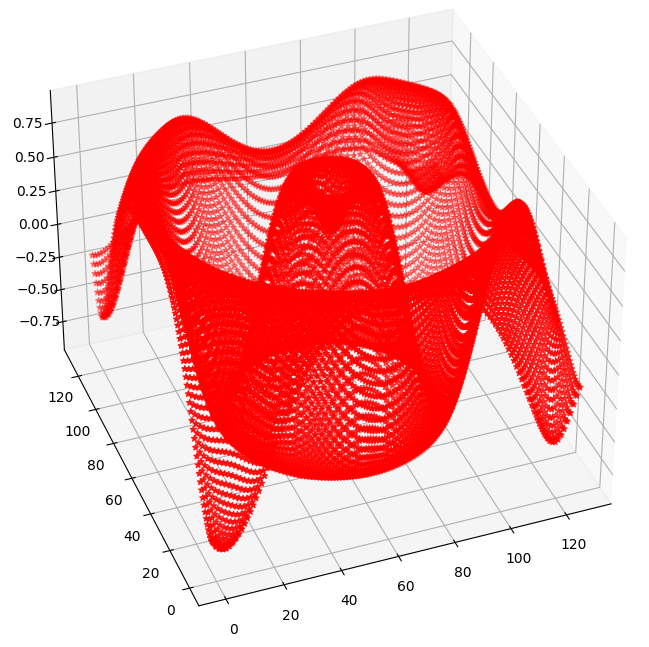
\includegraphics[width=\textwidth
   % ,height
  ]{Figure_2__16x8__res} 
  \caption{Восстановленная поверхность}
  \label{res_16_4}
\end{figure}
\FloatBarrier


\begin{figure}[h!]
  \centering
  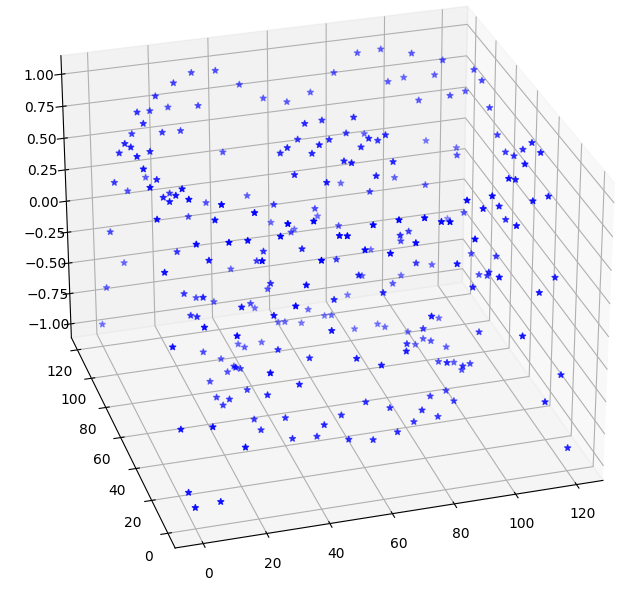
\includegraphics[width=\textwidth
   % ,height
  ]{Figure_2__16x8__in} 
  \caption{Исходные данные}
  \label{in_16_4}
\end{figure}
\FloatBarrier


%<Тут надо бы отметить что на рисунке видно что всё хорошо получилось >
%
%<Расскомментить и отредактировать общее заключение в файле paper\_func\_recv>

%%% Local Variables: 
%%% mode: latex
%%% TeX-master: "paper_func_recv"
%%% End: 



